\section{Используемые языки и технологии}

Так как предлагаемая функциональность представляет из себя расширение уже существующего компилятора формата protobuf ~--~ \textit{protoc}, то набор
используемых языков и технологий определяется уже существующей кодовой базой. Ниже перечислены факторы, оправдывающие выбор данных языков и технологий авторами компилятора:
\begin{itemize}
    \item кроссплатформенность ~--~ компилятор должен работать на тех же платформах, на которых предполагается сборка программного обеспечения, использующего protobuf;
    \item скорость выполнения ~--~ большое время компиляции задерживает процессы разработки, отладки и тестирования;
    \item компилируемость ~--~ бинарный файл компилятора легко распространять среди разработчиков.
\end{itemize}

\subsection{Язык программирования C++}

C++ представляет собой универсальный объектно-ориентированный язык программирования, разработанный Бьёрном Страуструпом в начале 1980-х годов. Он был создан на основе языка C с целью расширить его возможности и обеспечить разработку широкого спектра приложений, включая операционные системы, прикладные программы, драйверы устройств, встраиваемые системы, серверы и компьютерные игры.

Одной из ключевых особенностей C++ является его способность сочетать свойства как высокоуровневых, так и низкоуровневых языков программирования. Это делает его мощным инструментом в руках разработчиков, позволяя им гибко управлять системными ресурсами и одновременно использовать развитые средства абстракции\cite{modern_and_effective_cpp}.

C++ поддерживает различные парадигмы программирования, такие как процедурное, объектно-ориентированное и обобщённое программирование. Богатая стандартная библиотека языка включает в себя разнообразные контейнеры, алгоритмы, средства ввода-вывода, работы с регулярными выражениями и поддержку многопоточности. Это значительно упрощает разработку сложных программных систем, позволяя разработчикам использовать готовые, хорошо протестированные решения.

Эффективность и возможность низкоуровневого управления памятью делают C++ идеальным выбором для разработки высокопроизводительных приложений, требующих оптимизации использования системных ресурсов. Развитые средства объектно-ориентированного программирования, такие как классы, наследование, полиморфизм и инкапсуляция, позволяют создавать модульные и масштабируемые программные системы. Кроме того, поддержка обобщённого программирования посредством шаблонов обеспечивает гибкость и типобезопасность кода.

Несмотря на свою мощь, C++ также известен своей сложностью и крутой кривой обучения. Язык предоставляет множество низкоуровневых возможностей, что требует от разработчиков глубокого понимания принципов работы компьютера и эффективного управления ресурсами. Это может создавать определённые трудности, особенно для начинающих программистов.

В целом, C++ является одним из самых популярных и широко используемых языков программирования, применяемых в различных отраслях, таких как автомобилестроение, телекоммуникации, финансы и образование. Его сочетание мощности, гибкости и эффективности делает его незаменимым инструментом в арсенале современных разработчиков.

\subsection{Компилятор CLang}

Clang ~--~ это кроссплатформенный компилятор с открытым исходным кодом, созданный Apple и поддерживаемый 
сообществом LLVM. Он предназначен для компиляции языков C, C++, Objective-C и Objective-C++. 
Clang известен своей скоростью, точностью и поддержкой новейших функций языка.

Clang состоит из нескольких компонентов, каждый из которых играет важную роль в процессе компиляции:

\begin{itemize}
    \item лексический анализатор ~--~ преобразует исходный код в токены, которые представляют собой основные элементы языка;
    \item синтаксический анализатор ~--~ анализирует последовательность токенов, чтобы проверить их соответствие грамматике языка;
    \item семантический анализатор ~--~ проверяет семантическую правильность кода, включая типы данных, объявления переменных и операторы;
    \item промежуточное представление ~--~ преобразует код в промежуточное представление (IR), которое является абстрактным представлением кода, независимым от целевой платформы;
    \item оптимизатор ~--~ оптимизирует IR для повышения производительности кода;
    \item генератор кода ~--~ преобразует IR в машинный код для конкретной целевой платформы.
\end{itemize}

Clang обладает рядом преимуществ, которые делают его привлекательным выбором для разработки программного обеспечения:

\begin{itemize}
    \item скорость ~--~ Clang известен своей высокой скоростью компиляции, что особенно важно для больших проектов;
    \item точность ~--~ Clang обеспечивает точную диагностику ошибок, помогая разработчикам быстро находить и исправлять ошибки в своем коде;
    \item поддержка новейших функций языка ~--~ Clang поддерживает новейшие функции языков C, C++, Objective-C и Objective-C++, что позволяет разработчикам использовать самые передовые возможности;
    \item кроссплатформенность ~--~ Clang может компилировать код для различных платформ, включая Linux, macOS, Windows, iOS и Android;
    \item открытый исходный код ~--~ Clang ~--~ это проект с открытым исходным кодом, что означает, что его код доступен для проверки и модификации кем угодно;
    \item совместимость ~--~ Clang совместим с другими инструментами LLVM, что позволяет использовать его в комплексных рабочих процессах разработки.
\end{itemize}

Несмотря на свои преимущества, Clang имеет некоторые недостатки, которые следует учитывать:
\begin{itemize}
    \item сложность ~--~ Clang ~--~ это сложный инструмент, и его изучение может занять некоторое время;
    \item ограниченная поддержка некоторых функций ~--~ Clang может не поддерживать некоторые функции языков C и C++, особенно те, которые являются специфичными для определенных компиляторов или платформ.
\end{itemize}

Clang обладает рядом функций, которые отличают его от других компиляторов:

\begin{itemize}
    \item модульная архитектура ~--~ Clang имеет модульную архитектуру, что позволяет легко добавлять новые функции и расширения;
    \item статический анализ ~--~ Clang может выполнять статический анализ кода, выявляя потенциальные проблемы, такие как утечки памяти и незащищенные вызовы функций;
    \item автоматическое исправление ~--~ Clang может автоматически исправлять некоторые ошибки кода, что помогает разработчикам экономить время;
    \item поддержка расширений ~--~ Clang поддерживает расширения, которые позволяют разработчикам добавлять новые функции в язык.
\end{itemize}

Clang ~--~ это мощный и универсальный компилятор, который предлагает ряд преимуществ для разработки программного обеспечения.

\subsection{Система сборки CMake}
CMake ~--~ это инструмент для автоматизации процесса сборки и установки программного обеспечения. Он был разработан компанией Kitware и впервые использован в проекте ITK в 1999 году. CMake не занимается непосредственно сборкой, а генерирует файлы сборки на основе заранее написанного файла сценария CMakeLists.txt.
Основные возможности CMake:
\begin{itemize}
\item настраиваемая структура проекта ~--~ CMake находит общесистемные и пользовательские каталоги исполняемых файлов, файлов конфигураций и библиотек;
\item поддержка разных сред разработки ~--~ CMake создаёт файлы проектов для популярных интегрированных сред разработки, таких как Microsoft Visual Studio, Xcode и Eclipse CDT;
\item поддержка компиляторов ~--~ CMake определяет свойства, которые компилятор должен поддерживать для компиляции целевой программы или библиотеки.
\end{itemize}

Процесс сборки состоит из двух этапов:
\begin{itemize}
\item генерация стандартных файлов сборки из файлов конфигурации CMakeLists.txt;
\item использование системных инструментов сборки, таких как make, Ninja, для непосредственной компиляции программ.
\end{itemize}

CMake также предоставляет возможность создавать подпроекты, собирать их перед сборкой основного проекта и создавать цепочки зависимостей.

\subsection{Текстовый редактор NeoVim}

NeoVim ~--~ это современный текстовый редактор, основанный на Vim, который был создан с учётом современных требований и тенденций. Он предлагает улучшенную производительность, новые возможности и инструменты для комфортной работы с кодом.
NeoVim разработан с учётом принципов модульности и расширяемости, что позволяет пользователям легко добавлять и настраивать плагины и функции в соответствии со своими потребностями. Редактор также поддерживает работу с несколькими вкладками и окнами, что упрощает управление несколькими проектами одновременно.
Одной из ключевых особенностей NeoVim является использование Lua в качестве основного языка программирования. Это позволяет разработчикам создавать свои собственные плагины и расширения, которые могут быть интегрированы с редактором без необходимости знания языка программирования VimScript.
Ещё одной важной особенностью NeoVim является поддержка нескольких режимов работы. В режиме Ex команды выполняются напрямую, а в режиме Vi команды интерпретируются и обрабатываются редактором. Это обеспечивает гибкость и удобство работы с различными типами кода и файлами.
Редактор имеет встроенную систему автозаполнения, которая помогает разработчикам быстрее и точнее писать код.
В целом, NeoVim представляет собой мощный и удобный текстовый редактор, который подходит для разработчиков всех уровней опыта и специализации. Благодаря своей гибкости, модульности и поддержке современных технологий, он становится незаменимым инструментом для работы с кодом в современном мире разработки программного обеспечения.

\subsection{Google Test}
Google Test (также известный как GTest) ~--~ это фреймворк для модульного тестирования, разработанный и используемый компанией Google\cite{how_google_tests_software}. Он является одним из самых популярных фреймворков тестирования для C++ и широко используется в различных проектах, включая код Google и сторонние приложения.

Основные характеристики Google Test:
\begin{itemize}
    \item простота использования ~--~ Google Test обладает простым и понятным интерфейсом, что делает его доступным для разработчиков с различным уровнем опыта;
    \item гибкость ~--~ Google Test поддерживает различные стили написания тестов, такие как тестовые фикстуры, тестовые кейсы и тестовые группы;
    \item расширяемость ~--~ Google Test позволяет разработчикам создавать собственные расширения и фикстуры для тестирования различных сценариев;
    \item интеграция с CI/CD ~--~ Google Test легко интегрируется с системами непрерывной интеграции и непрерывной доставки (CI/CD), что позволяет автоматизировать процесс тестирования.
    \item cовместимость ~--~ Google Test совместим с различными компиляторами C++ и платформами.
\end{itemize}

Google Test состоит из следующих основных компонентов:

\begin{itemize}
    \item тестовая фикстура ~--~ это класс, который содержит зафиксированные тестовые данные;
    \item тестовый кейс ~--~ это функция, которая проверяет определенную функциональность приложения;
    \item тестовая группа ~--~ это группа тестовых кейсов, связанных между собой;
    \item ASSERT\_ макросы ~--~ Google Test предоставляет набор макросов ASSERT\_, которые используются для проверки условий в тестовых кейсах;
    \item EXPECT\_ макросы ~--~ Google Test предоставляет набор макросов EXPECT\_, которые используются для проверки ожидаемого поведения приложения в тестовых кейсах.
\end{itemize}

Пример использования Google Test приведён в листинге \ref{sec_testing:code:gtest}.
\pagebreak
\begin{lstlisting}[style=CodeListing, caption={Пример тестов, описанных с помощью GTest}, label=sec_testing:code:gtest]
#include "gtest/gtest.h"

class MyMathTest : public ::testing::Test {
protected:
  // Setup function
  virtual void SetUp() override {
    // Initialize variables
  }

  // Teardown function
  virtual void TearDown() override {
    // Clean up resources
  }
};

TEST_F(MyMathTest, Add) {
  int a = 5;
  int b = 3;
  int expected_sum = 8;

  int actual_sum = MyMath::Add(a, b);

  EXPECT_EQ(expected_sum, actual_sum);
}

TEST_F(MyMathTest, Subtract) {
  int a = 10;
  int b = 5;
  int expected_difference = 5;

  int actual_difference = MyMath::Subtract(a, b);

  EXPECT_EQ(expected_difference, actual_difference);
}
\end{lstlisting}

Преимущества Google Test:
\begin{itemize}
    \item простота и понятность;
    \item эффективность;
    \item надежность;
    \item сокращение времени разработки;
    \item повышение качества кода.
\end{itemize}

\subsection{Perf и flamegraph}

Perf - это инструмент для анализа производительности, который был добавлен в ядро Linux версии 2.6.31 в 2009 году.
Он использует отслеживание стека ядра в режиме реального времени для отсления выполнения программ и может предоставить 
достаточно подробную информацию, чтобы найти узкие места в производительнои расставить приоритеты в оптимизации работы программ.

\subsubsection{Установка} 

На некоторых системах Perf может быть установлен по умолчанию, но это не всегда так.
К примеру, на Debian Buster, предустановлены только пользовательские программы, поэтому соответствующие инструменты ядра все еще нужно установливать вручную.
Для ручной установки утилиты следует ввести команду, представленную в листинге \ref{code:perf_install}.

\begin{lstlisting}[style=CodeListing, caption={Установка утилиты perf в ОС Linux}, label=code:perf_install]
sudo apt install linux-perf # or
sudo apt install linux-perf-5.8
\end{lstlisting}

После установки можно попробовать запустить perf, но с большой вероятностью будет получена либо ошибка, представленная в листинге \ref{sec_tech:code:perf_err1}, либо ошибка, представленная в листинге \ref{sec_tech:code:perf_err2}.

\noindent\begin{minipage}{\linewidth}
\begin{lstlisting}[style=CodeListing, label=sec_tech:code:perf_err1, caption={Первый вариант ошибки, встречающейся после установки утилиты}]
\$> perf record
Error:
You may not have permission to collect stats.
Consider tweaking /proc/sys/kernel/perf_event_paranoid:
 -1 - Not paranoid at all
  0 - Disallow raw tracepoint access for unpriv
  1 - Disallow cpu events for unpriv
  2 - Disallow kernel profiling for unpriv
\end{lstlisting}

\begin{lstlisting}[style=CodeListing, label=sec_tech:code:perf_err2, caption={Второй вариант ошибки, встречающейся после установки утилиты}]
Error:
Access to performance monitoring and observability operations is limited.
Consider adjusting /proc/sys/kernel/perf_event_paranoid setting to open
access to performance monitoring and observability operations for processes
without CAP_PERFMON, CAP_SYS_PTRACE or CAP_SYS_ADMIN Linux capability.
More information can be found at 'Perf events and tool security' document:
https://www.kernel.org/doc/html/latest/admin-guide/perf-security.html
perf_event_paranoid setting is 3:
  -1: Allow use of (almost) all events by all users
      Ignore mlock limit after perf_event_mlock_kb without CAP_IPC_LOCK
>= 0: Disallow raw and ftrace function tracepoint access
>= 1: Disallow CPU event access
>= 2: Disallow kernel profiling
To make the adjusted perf_event_paranoid setting permanent preserve it
in /etc/sysctl.conf (e.g. kernel.perf_event_paranoid = <setting>)
\end{lstlisting}
\end{minipage}

Это связано с тем, что по соображениям безопасности ядро Linux по умолчанию запрещает непривилегированным пользователям 
осуществлять мониторинг производительности системы. Существует несколько способов решения этой проблемы:

\begin{itemize}
    \item изменить параметр ядра \textit{kernel.perf\_event\_paranoid};
    \item добавить разрешение \textit{CAP\_PERFMON} к perf;
    \item использовать root-пользователя для мониторинга производительности.
\end{itemize}

Наиболее правильным с точки зрения философии операционной системы Linux является первый способ, 
так как не рекомендуется запускать perf с root-пользователем из соображений безопасности.

Есть два способа изменить параметр \textit{kernel.perf\_event\_paranoid}.
Первый метод временный и требует повторения действий после перезагрузки системы, но требует меньших усилий.
Он состоит в выполнении одной из команд, представленных в листинге \ref{sec_tech:code:change_perf_event_paranoid}.

\begin{lstlisting}[style=CodeListing, label=sec_tech:code:change_perf_event_paranoid, caption={Способы изменения параметра}]
sudo sh -c "echo -1 > /proc/sys/kernel/perf_event_paranoid"

sudo sysctl -w kernel.perf\_event\_paranoid=-1
\end{lstlisting}

Второй метод ~--~ изменить файл конфигурации sysctl, который находится по пути \textit{/etc/sysctl.conf}.
Команды для выполнения данной процедуры представлены в листинге \ref{sec_tech:code:change_sysctl}.

\begin{lstlisting}[style=CodeListing, label=sec_tech:code:change_sysctl, caption={Правка файла конфигурации sysctl}]
sudo sh -c 'echo "kernel.perf_event_paranoid=-1" >> /etc/sysctl.conf'
sudo sysctl -p
\end{lstlisting}

После этого ядро разрешит непривилегированным пользователям использовать интерфейсы в разделе ядра perf.

\subsubsection{Использование} 

Существует несколько распространенных способов использования perf. 
Первый из них ~--~ получить простое грубое представление о том, как программа использует аппаратные ресурсы.
В листинге \ref{} представлен пример получения такого отчёта для команды \textit{ls}.

\pagebreak
\begin{lstlisting}[style=CodeListing, label=sec_tech:code:pref_stat, caption={Пример использования команды perf stat}]
\$> perf stat ls

<stdout>
Performance counter stats for 'ls':

apache
Copy
          1.87 msec task-clock                #    0.411 CPUs utilized
            11      context-switches          #    0.006 M/sec
             0      cpu-migrations            #    0.000 K/sec
            94      page-faults               #    0.050 M/sec
     2,771,746      cycles                    #    1.479 GHz
     1,534,926      instructions              #    0.55  insn per cycle
       317,631      branches                  #  169.519 M/sec
        15,169      branch-misses             #    4.78% of all branches

   0.004553499 seconds time elapsed

   0.003498000 seconds user
   0.000000000 seconds sys
\end{lstlisting}

Второй способ позволяет делать детальный анализ процентного соотношения времени выполнения каждой функции программы, 
а также процентного соотношения времени, затрачиваемого на каждую инструкцию в этих функциях, что позволяет 
получить точное представление об использовании процессорных ресурсов узким местом времени выполнения программы. Для этого
достаточно выполнить команду \textit{perf record}, чтобы утилита начала отслеживать выполнение, а после завершения работы программы
вызвать \textit{perf report}, как продемонстрировано в листинге \ref{}

\begin{lstlisting}[style=CodeListing, label=sec_tech:code:perf_record_report, caption={Пример использования команд perf record и perf report}]
perf record <program>
perf report
\end{lstlisting}

Команда \textit{perf record} представляет отчёт, пример которого приведён на рисунке \ref{sec_technologies:fig:perf_report_example}.
\begin{figure}[H]
    \centering
    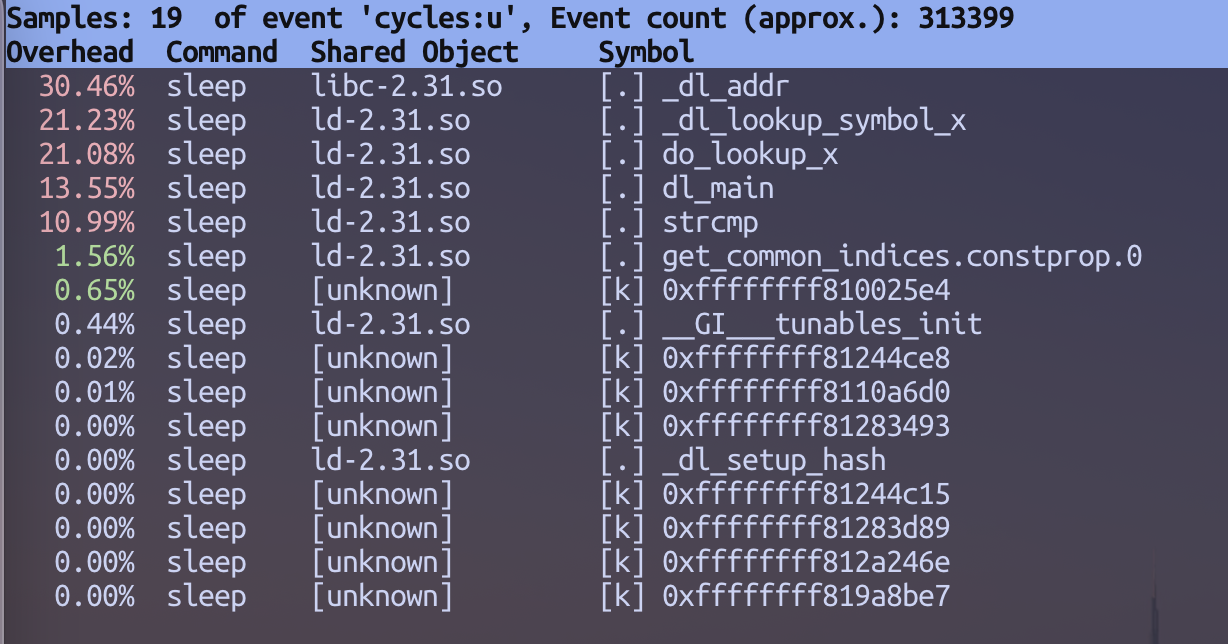
\includegraphics[width=0.85\linewidth]{\commonSecPathPrefix/sec_technologies_attachments/perf_report_example.png}
    \caption{Отчёт утилиты perf о работе команды sleep}
    \label{sec_technologies:fig:perf_report_example}
\end{figure}

Иногда, если опция отладки выключена во время компиляции (например, в случае компилятора \textit{gcc}, не выставлен флаг \textit{-g}),
вероятно, что perf не сможет получить все человекочитаемые имена вызываемых методов, что сделает статистику 
нечитаемой и лишит возможности какого-либо удобного анализа результатов. 
В этом случае можно указать один из методов трассировки стека вызовов, доступных в утилите.
Пример такого вызова команды \textit{perf record} представлен в листинге \ref{sec_technologies:code:pref_record_modes}.

\begin{lstlisting}[style=CodeListing, label=sec_technologies:code:pref_record_modes, caption={Вызов команды perf record с указанием метода трассировки стека вызовов}]
perf record --call-graph <method> <program>
\end{lstlisting}

Всего доступно три метода трассировки.
\begin{enumerate}
    \item fp ~--~ наименнее детальный, порождает самый малый из всех файл логов наблюдений и имеет самое незначительное влияние на производительность тестируемого приложения.
    \item lbr ~--~ более детальный метод, порождающий соответственно больший файл с наблюдениями и имеющий небольшое, но заметное влияние на производительность тестируемого приложения.
    \item dwarf ~--~ наиболее детальный метод трассировки. Может порождать файлы наблюдений, достигающие размеров в 10 гигабайт за минуту наблюдений. Сильно влияет на производительность исследуемого приложения.
\end{enumerate}

\pagebreak
Флеймграф (Flamegraph) ~--~ это инструмент визуализации результатов профилирующих утилит. Он представляет собой древовидную диаграмму, где каждый узел представляет собой функцию, а его ширина пропорциональна времени, затрачиваемому на выполнение этой функции. Флеймграфы позволяют разработчикам быстро и легко определить, какие части кода занимают больше всего времени, что помогает им оптимизировать производительность приложения.

Флеймграфы были впервые представлены в статье 2004 года <<Visualizing Performance with Flame Graphs>> авторства Б. Л. Коллинза. 
С тех пор они стали популярным инструментом для профилирования производительности в различных областях, включая программное обеспечение, системное администрирование и научные вычисления.

Флеймграфы позволяют визуализировать стек вызовов гораздо более наглядным образом. Они дают представление 
о производительности кода и позволяют эффективно отлаживать его, углубляясь в источник ошибки. 

Визуализация представлена в виде древовидной структуры, где узел соединяется с другим узлом для отображения их родительско-дочерних отношений. 
Такое отношение соответствует стеку вызовов, где одна функция вызывает другую, пока не дойдет до последней функции в стеке. 
Затем древовидная структура преобразуется в набор блоков, налагаемых друг на друга в соответствии с их отношениями. Результат этих операций называется флеймграфом.
На рисунке \ref{sec_tech:fig:flamegraph_tree} представлен пример представления стека вызовов программы в виде древовидной структуры.

\begin{figure}[H]
    \centering
    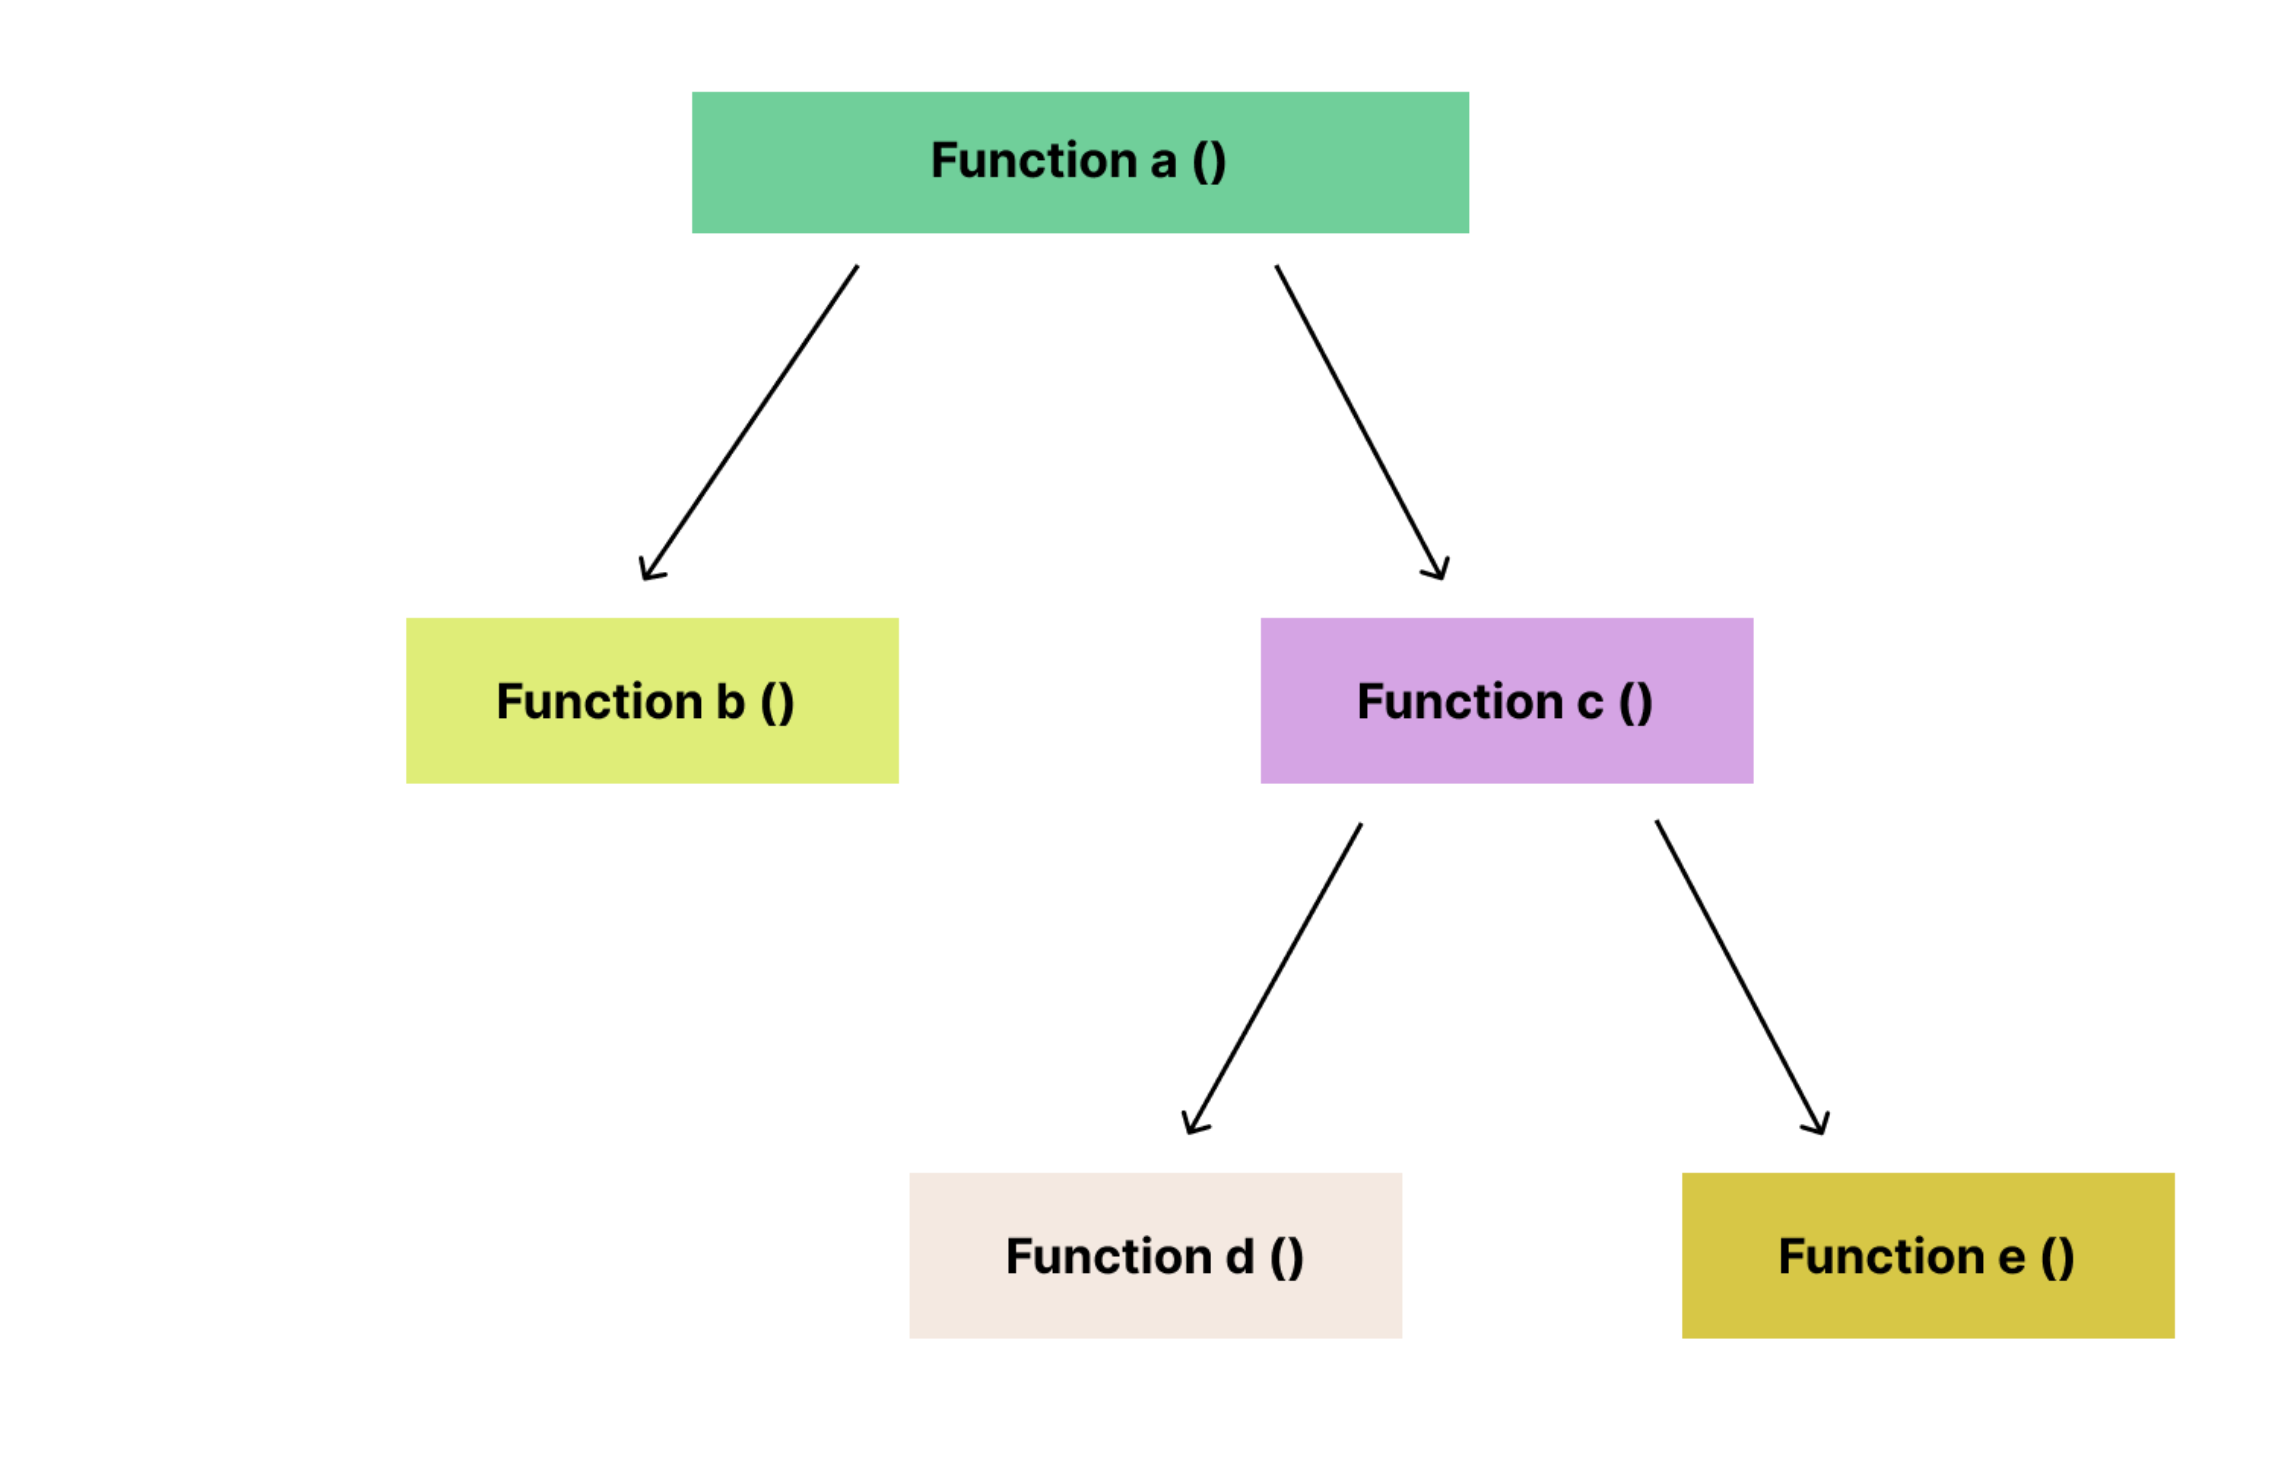
\includegraphics[width=0.85\linewidth]{\commonSecPathPrefix/sec_technologies_attachments/call_stack_tree_example.png}
    \caption{Пример представления стека вызовов программы в виде дерева}
    \label{sec_tech:fig:flamegraph_tree}
\end{figure}

На рисунке \ref{sec_tech:fig:flamegraph_example_from_tree} представлен флеймграф, построенный на основе дерева на рисунке \ref{sec_tech:fig:flamegraph_tree}.

\begin{figure}[H]
    \centering
    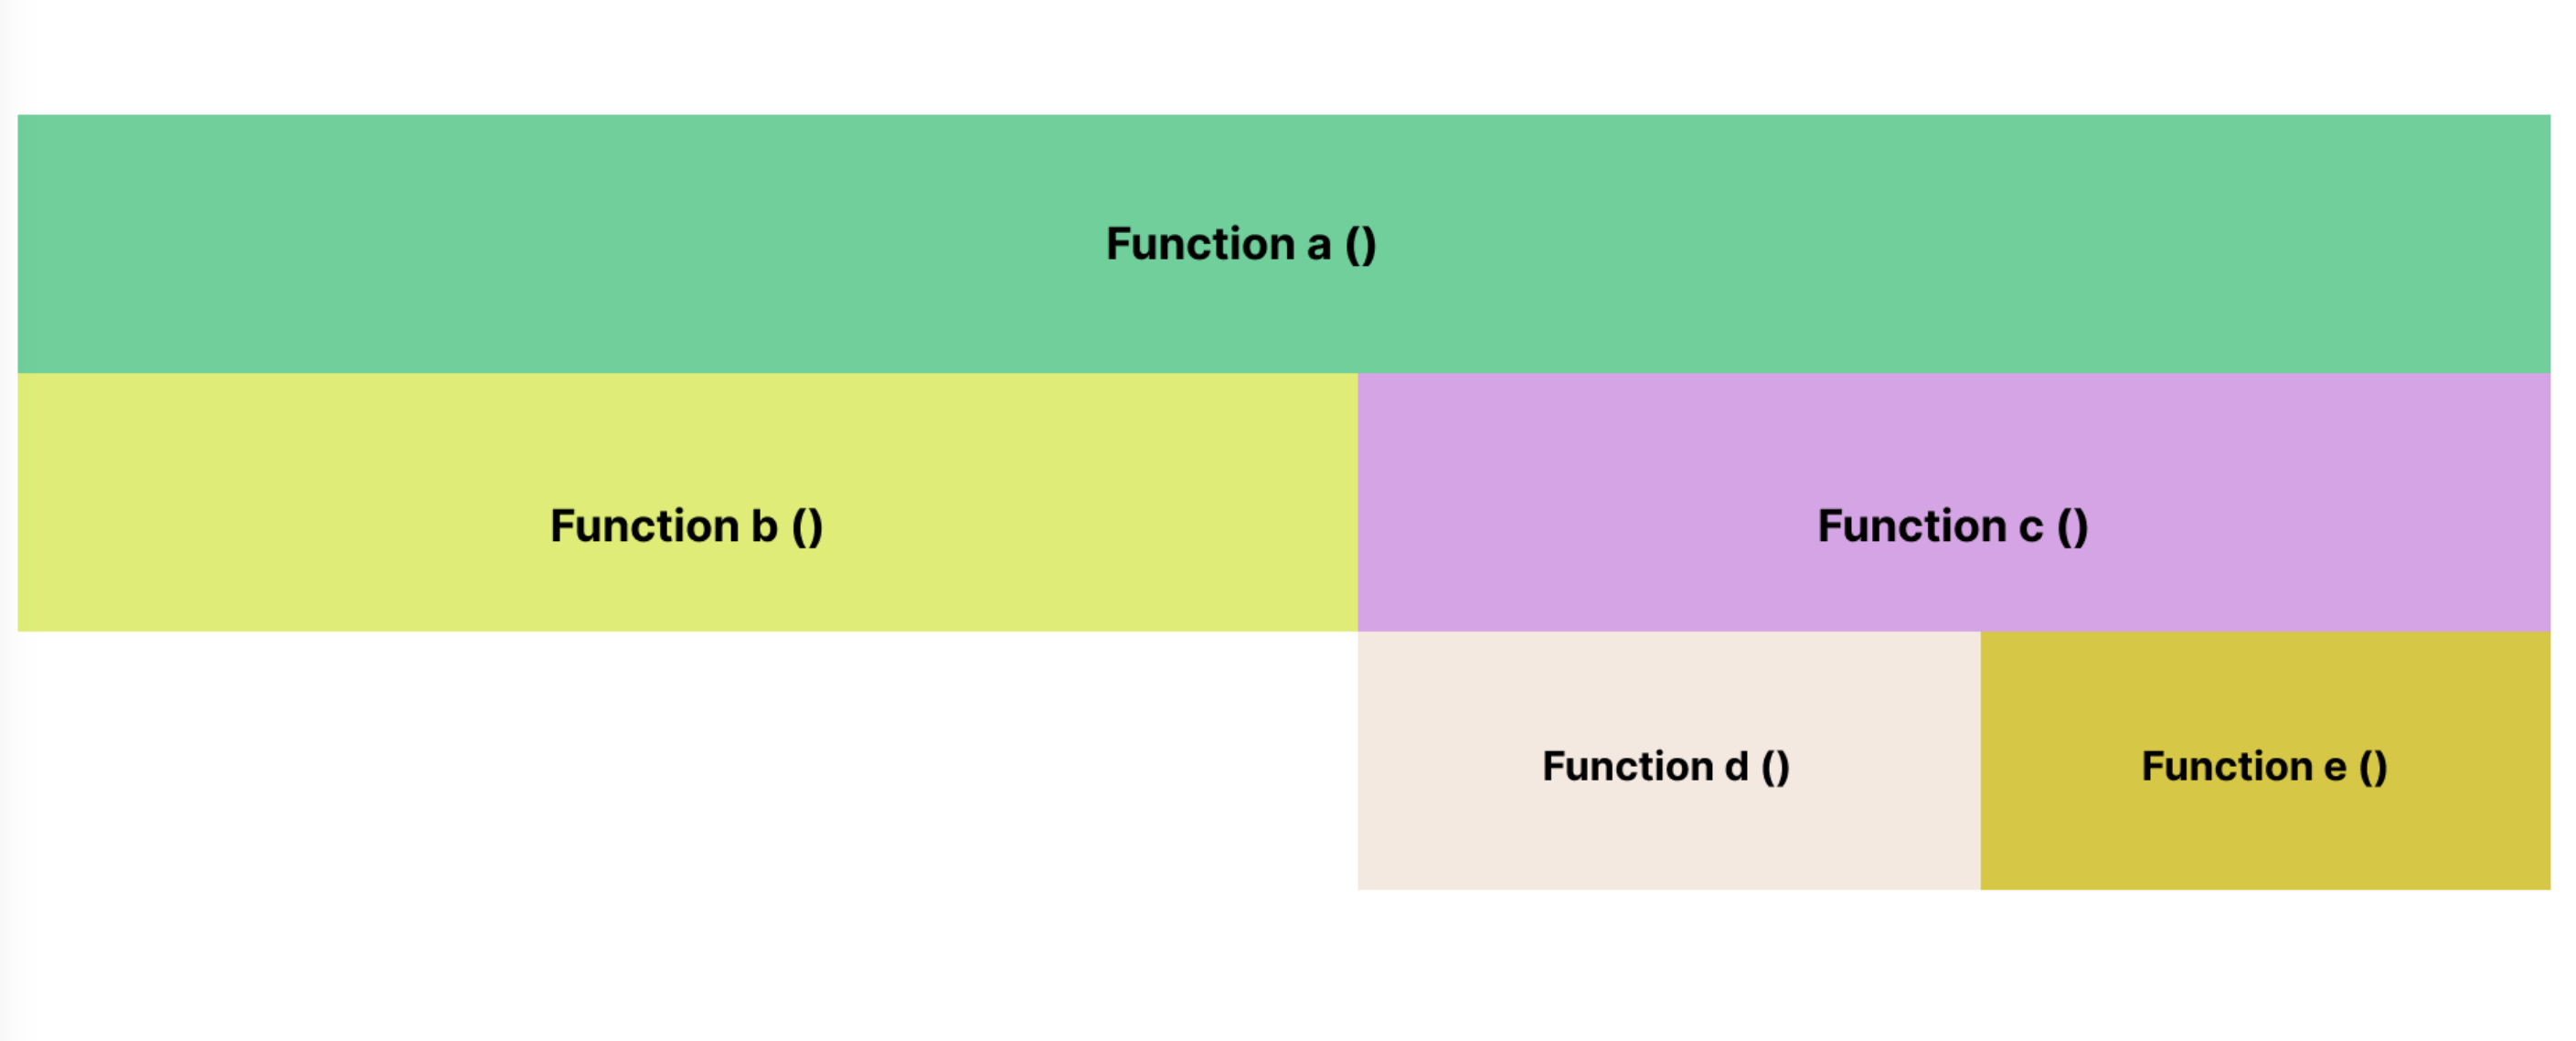
\includegraphics[width=0.85\linewidth]{\commonSecPathPrefix/sec_technologies_attachments/call_stack_flame_example.png}
    \caption{Пример представления стека вызовов в виде простейшего флеймграфа}
    \label{sec_tech:fig:flamegraph_example_from_tree}
\end{figure}

К сценариям использования флеймграфов можно отнести отладку просадок производительности после выхода новой версии ПО,
резкие скачки потребления ресурсов процессора, когда приложение уже используется аудиторией, анализ приложений с целью
их дальнейшей оптимизации.
Флеймграфы - лучший способ визуализировать данные о производительности.
Они позволяют получить полное представление о вычислительных ресурсах и их использовании на одной панели. 
Когда что-то идет не так, вы можете быстро определить разницу между идеальным <<эффективным>> состоянием и ошибочным <<неэффективным>> состоянием.

Построение флеймграфа состоит из трёх шагов:
\begin{enumerate}
    \item Сбор системных событий (в том числе с помощью рассмотренной ранее утилиты \textit{perf}).
    \item Сворачивание стеков вызвов. На этом шаге события, собранные ранее, структурируются и группируются для удобного отображения.
    \item Визуализация. Утилита создаёт файл представления (зачастую в формате \textit{svg}) на основе структурированных на предыдущем шаге событий.
\end{enumerate}

Существует множество инструментов для постоения флеймграфов, однако одной из самых распространённых является \textit{flamegraph.pl}.
Это инструмент с открытым исходным кодом, написанный на языке Pearl. Его преимуществами являются легковесность, простота установки и использования,
удобный формат вывода. Утилита создаёт кликабельные флеймграфы. Это означает, что при клике на определённый метод можно более подробно изучить распределение
затрат процессора именно внутри него.
